\documentclass{standalone}
\usepackage{tikz}
\usetikzlibrary{patterns, positioning}

\begin{document}
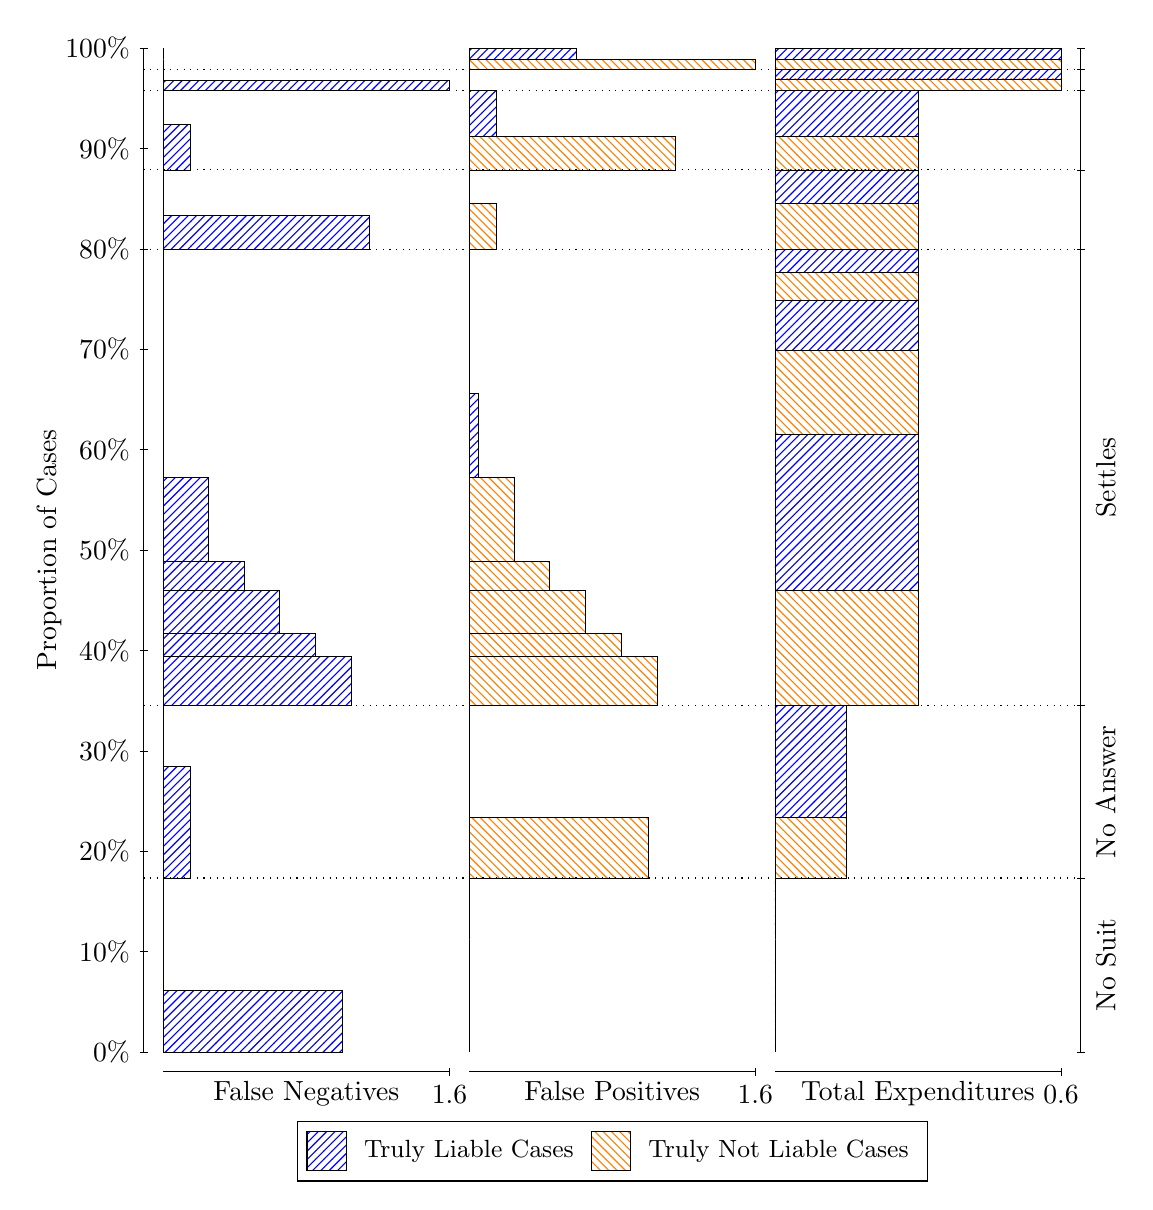
\begin{tikzpicture}
\draw[black, very thin] (1.5,1.75) -- (1.5,14.5);
\node[rotate=90, anchor=center] at (0.3, 8.125) {Proportion of Cases};
\draw[black, very thin] (1.45,1.75) -- (1.55,1.75);
\node[anchor=east] at (1.45, 1.75) {0\%};
\draw[black, very thin] (1.45,3.025) -- (1.55,3.025);
\node[anchor=east] at (1.45, 3.025) {10\%};
\draw[black, very thin] (1.45,4.3) -- (1.55,4.3);
\node[anchor=east] at (1.45, 4.3) {20\%};
\draw[black, very thin] (1.45,5.575) -- (1.55,5.575);
\node[anchor=east] at (1.45, 5.575) {30\%};
\draw[black, very thin] (1.45,6.85) -- (1.55,6.85);
\node[anchor=east] at (1.45, 6.85) {40\%};
\draw[black, very thin] (1.45,8.125) -- (1.55,8.125);
\node[anchor=east] at (1.45, 8.125) {50\%};
\draw[black, very thin] (1.45,9.4) -- (1.55,9.4);
\node[anchor=east] at (1.45, 9.4) {60\%};
\draw[black, very thin] (1.45,10.675) -- (1.55,10.675);
\node[anchor=east] at (1.45, 10.675) {70\%};
\draw[black, very thin] (1.45,11.95) -- (1.55,11.95);
\node[anchor=east] at (1.45, 11.95) {80\%};
\draw[black, very thin] (1.45,13.225) -- (1.55,13.225);
\node[anchor=east] at (1.45, 13.225) {90\%};
\draw[black, very thin] (1.45,14.5) -- (1.55,14.5);
\node[anchor=east] at (1.45, 14.5) {100\%};

\draw[black, very thin] (13.4,1.75) -- (13.4,14.5);
\draw[black, very thin] (13.35,1.75) -- (13.45,1.75);
\node[anchor=west] at (13.35, 1.75) {};
\draw[black, very thin] (13.35,3.9589) -- (13.45,3.9589);
\node[anchor=west] at (13.35, 3.9589) {};
\draw[black, very thin] (13.35,6.1483) -- (13.45,6.1483);
\node[anchor=west] at (13.35, 6.1483) {};
\draw[black, very thin] (13.35,11.943) -- (13.45,11.943);
\node[anchor=west] at (13.35, 11.943) {};
\draw[black, very thin] (13.35,12.953) -- (13.45,12.953);
\node[anchor=west] at (13.35, 12.953) {};
\draw[black, very thin] (13.35,13.963) -- (13.45,13.963);
\node[anchor=west] at (13.35, 13.963) {};
\draw[black, very thin] (13.35,14.231) -- (13.45,14.231);
\node[anchor=west] at (13.35, 14.231) {};
\draw[black, very thin] (13.35,14.5) -- (13.45,14.5);
\node[anchor=west] at (13.35, 14.5) {};

\draw[black, very thin, pattern color=blue, pattern=north east lines] (1.75,1.75) rectangle (4.0208,2.5285);
\draw[black, very thin, pattern color=orange, pattern=north west lines] (1.75,2.5285) rectangle (1.75,3.9589);
\draw[black, very thin, pattern color=blue, pattern=north east lines] (1.75,3.9589) rectangle (2.0906,5.3796);
\draw[black, very thin, pattern color=orange, pattern=north west lines] (1.75,5.3796) rectangle (1.75,6.1483);
\draw[black, very thin, pattern color=blue, pattern=north east lines] (1.75,6.1483) rectangle (4.1344,6.7788);
\draw[black, very thin, pattern color=blue, pattern=north east lines] (1.75,6.7788) rectangle (3.6802,7.0661);
\draw[black, very thin, pattern color=blue, pattern=north east lines] (1.75,7.0661) rectangle (3.226,7.6154);
\draw[black, very thin, pattern color=blue, pattern=north east lines] (1.75,7.6154) rectangle (2.7719,7.9774);
\draw[black, very thin, pattern color=blue, pattern=north east lines] (1.75,7.9774) rectangle (2.3177,9.0454);
\draw[black, very thin, pattern color=orange, pattern=north west lines] (1.75,9.0454) rectangle (1.75,11.943);
\draw[black, very thin, pattern color=blue, pattern=north east lines] (1.75,11.943) rectangle (4.3615,12.37);
\draw[black, very thin, pattern color=orange, pattern=north west lines] (1.75,12.37) rectangle (1.75,12.953);
\draw[black, very thin, pattern color=blue, pattern=north east lines] (1.75,12.953) rectangle (2.0906,13.535);
\draw[black, very thin, pattern color=orange, pattern=north west lines] (1.75,13.535) rectangle (1.75,13.963);
\draw[black, very thin, pattern color=blue, pattern=north east lines] (1.75,13.963) rectangle (5.3833,14.085);
\draw[black, very thin, pattern color=orange, pattern=north west lines] (1.75,14.085) rectangle (1.75,14.231);
\draw[black, very thin, pattern color=orange, pattern=north west lines] (1.75,14.231) rectangle (1.75,14.354);
\draw[black, very thin, pattern color=blue, pattern=north east lines] (1.75,14.354) rectangle (1.75,14.5);
\draw[black, very thin, pattern color=orange, pattern=north west lines] (5.6333,1.75) rectangle (5.6333,3.1805);
\draw[black, very thin, pattern color=blue, pattern=north east lines] (5.6333,3.1805) rectangle (5.6333,3.9589);
\draw[black, very thin, pattern color=orange, pattern=north west lines] (5.6333,3.9589) rectangle (7.9042,4.7276);
\draw[black, very thin, pattern color=blue, pattern=north east lines] (5.6333,4.7276) rectangle (5.6333,6.1483);
\draw[black, very thin, pattern color=orange, pattern=north west lines] (5.6333,6.1483) rectangle (8.0177,6.7788);
\draw[black, very thin, pattern color=orange, pattern=north west lines] (5.6333,6.7788) rectangle (7.5635,7.0661);
\draw[black, very thin, pattern color=orange, pattern=north west lines] (5.6333,7.0661) rectangle (7.1094,7.6154);
\draw[black, very thin, pattern color=orange, pattern=north west lines] (5.6333,7.6154) rectangle (6.6552,7.9774);
\draw[black, very thin, pattern color=orange, pattern=north west lines] (5.6333,7.9774) rectangle (6.201,9.0454);
\draw[black, very thin, pattern color=blue, pattern=north east lines] (5.6333,9.0454) rectangle (5.7469,10.113);
\draw[black, very thin, pattern color=blue, pattern=north east lines] (5.6333,10.113) rectangle (5.6333,11.943);
\draw[black, very thin, pattern color=orange, pattern=north west lines] (5.6333,11.943) rectangle (5.974,12.525);
\draw[black, very thin, pattern color=blue, pattern=north east lines] (5.6333,12.525) rectangle (5.6333,12.953);
\draw[black, very thin, pattern color=orange, pattern=north west lines] (5.6333,12.953) rectangle (8.2448,13.381);
\draw[black, very thin, pattern color=blue, pattern=north east lines] (5.6333,13.381) rectangle (5.974,13.963);
\draw[black, very thin, pattern color=orange, pattern=north west lines] (5.6333,13.963) rectangle (5.6333,14.109);
\draw[black, very thin, pattern color=blue, pattern=north east lines] (5.6333,14.109) rectangle (5.6333,14.231);
\draw[black, very thin, pattern color=orange, pattern=north west lines] (5.6333,14.231) rectangle (9.2667,14.354);
\draw[black, very thin, pattern color=blue, pattern=north east lines] (5.6333,14.354) rectangle (6.9958,14.5);
\draw[black, very thin, pattern color=orange, pattern=north west lines] (9.5167,1.75) rectangle (9.5167,3.1805);
\draw[black, very thin, pattern color=blue, pattern=north east lines] (9.5167,3.1805) rectangle (9.5167,3.9589);
\draw[black, very thin, pattern color=orange, pattern=north west lines] (9.5167,3.9589) rectangle (10.425,4.7276);
\draw[black, very thin, pattern color=blue, pattern=north east lines] (9.5167,4.7276) rectangle (10.425,6.1483);
\draw[black, very thin, pattern color=orange, pattern=north west lines] (9.5167,6.1483) rectangle (11.333,7.6154);
\draw[black, very thin, pattern color=blue, pattern=north east lines] (9.5167,7.6154) rectangle (11.333,9.5947);
\draw[black, very thin, pattern color=orange, pattern=north west lines] (9.5167,9.5947) rectangle (11.333,10.663);
\draw[black, very thin, pattern color=blue, pattern=north east lines] (9.5167,10.663) rectangle (11.333,11.293);
\draw[black, very thin, pattern color=orange, pattern=north west lines] (9.5167,11.293) rectangle (11.333,11.655);
\draw[black, very thin, pattern color=blue, pattern=north east lines] (9.5167,11.655) rectangle (11.333,11.943);
\draw[black, very thin, pattern color=orange, pattern=north west lines] (9.5167,11.943) rectangle (11.333,12.525);
\draw[black, very thin, pattern color=blue, pattern=north east lines] (9.5167,12.525) rectangle (11.333,12.953);
\draw[black, very thin, pattern color=orange, pattern=north west lines] (9.5167,12.953) rectangle (11.333,13.381);
\draw[black, very thin, pattern color=blue, pattern=north east lines] (9.5167,13.381) rectangle (11.333,13.963);
\draw[black, very thin, pattern color=orange, pattern=north west lines] (9.5167,13.963) rectangle (13.15,14.109);
\draw[black, very thin, pattern color=blue, pattern=north east lines] (9.5167,14.109) rectangle (13.15,14.231);
\draw[black, very thin, pattern color=orange, pattern=north west lines] (9.5167,14.231) rectangle (13.15,14.354);
\draw[black, very thin, pattern color=blue, pattern=north east lines] (9.5167,14.354) rectangle (13.15,14.5);
\draw[black, dotted] (1.5,3.9589) -- (13.4,3.9589);
\draw[black, dotted] (1.5,6.1483) -- (13.4,6.1483);
\draw[black, dotted] (1.5,11.943) -- (13.4,11.943);
\draw[black, dotted] (1.5,12.953) -- (13.4,12.953);
\draw[black, dotted] (1.5,13.963) -- (13.4,13.963);
\draw[black, dotted] (1.5,14.231) -- (13.4,14.231);
\draw[black, very thin] (1.75,1.5) -- (5.3833,1.5);
\node[anchor=north] at (3.5667, 1.5) {False Negatives};
\draw[black, very thin] (5.3833,1.45) -- (5.3833,1.55);
\node[anchor=north] at (5.3833, 1.45) {1.6};

\draw[black, very thin] (5.6333,1.5) -- (9.2667,1.5);
\node[anchor=north] at (7.45, 1.5) {False Positives};
\draw[black, very thin] (9.2667,1.45) -- (9.2667,1.55);
\node[anchor=north] at (9.2667, 1.45) {1.6};

\draw[black, very thin] (9.5167,1.5) -- (13.15,1.5);
\node[anchor=north] at (11.333, 1.5) {Total Expenditures};
\draw[black, very thin] (13.15,1.45) -- (13.15,1.55);
\node[anchor=north] at (13.15, 1.45) {0.6};

\node[black, centered, rotate=90] at (13.72, 2.8545) {No Suit};
\node[black, centered, rotate=90] at (13.72, 5.0536) {No Answer};
\node[black, centered, rotate=90] at (13.72, 9.0454) {Settles};





\draw (7.449999999999999,1.5) node[draw=none] (baseCoordinate) {};
\begin{scope}[align=center]
        \matrix[scale=0.5, draw=black, below=0.5cm of baseCoordinate, nodes={draw}, column sep=0.1cm]{
            \node[rectangle, draw, minimum width=0.5cm, minimum height=0.5cm, pattern=north east lines, pattern color=blue] {}; &
            \node[draw=none, font=\small] (B) {Truly Liable Cases}; &
            \node[rectangle, draw, minimum width=0.5cm, minimum height=0.5cm, pattern=north west lines, pattern color=orange] {}; &
            \node[draw=none, font=\small] (B) {Truly Not Liable Cases}; \\
            };
\end{scope}

\end{tikzpicture}
\end{document}